%---------------------------------------------------------------------
%
%                          PeptideAtlas 2
%
%---------------------------------------------------------------------

\begin{otherlanguage}{british}

\chapter*{\href{http://www.ncbi.nlm.nih.gov/pubmed/26493587}{A comprehensive \textit{Candida albicans} PeptideAtlas build enables deep proteome coverage}}

\addcontentsline{toc}{chapter}{A comprehensive \textit{Candida albicans} PeptideAtlas build enables \\ deep proteome coverage}

\addcontentsline{lof}{chapter}{A comprehensive \textit{Candida albicans} PeptideAtlas build enables \\ deep proteome coverage}

\addcontentsline{lot}{chapter}{A comprehensive \textit{Candida albicans} PeptideAtlas build enables \\ deep proteome coverage}


%\renewcommand{\headrulewidth}{0pt}
\cabeceraEspecial{An extended, enhanced \textit{\mbox{C. albicans}} PeptideAtlas build}

\subsubsection*{Vital Vialas, Zhi Sun, Jose A. Reales Calder\'on, Mar\'ia L. Hern\'aez, Vanessa Casas, Montserrat Carrascal, Joaqu\'in Abi\'an, Luc\'ia Monteoliva, Eric W. Deutsch, Robert L. Moritz, Concha Gil}
\subsubsection*{Journal of Proteomics 2015, In Press, Available online 19 October 2015}
%doi:	10.1016/j.jprot.2015.10.019

\bigskip
\hfill
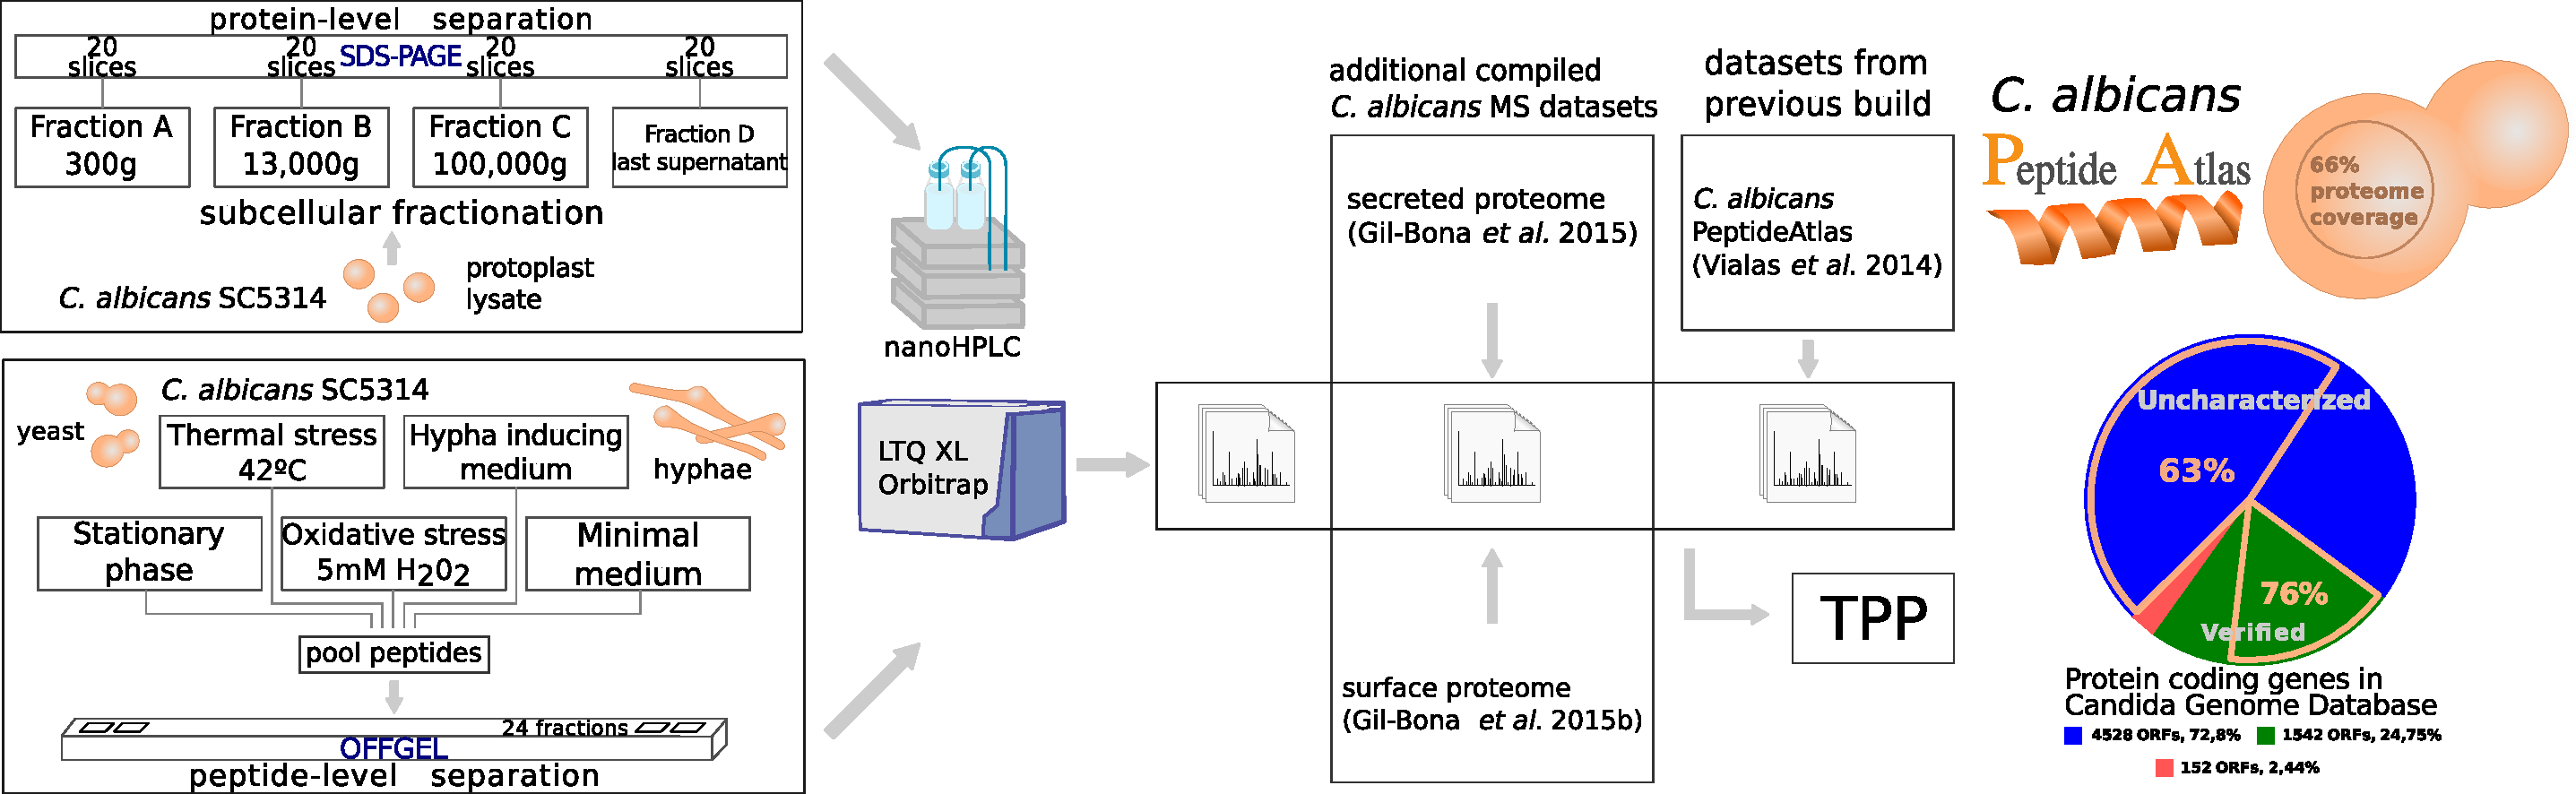
\includegraphics[width=1\textwidth]{Imagenes/Vectorial/graphical_abstract_PeptideAtlas2}




\newpage


\chapter*{Abstract}
To provide new and expanded proteome documentation of the opportunistically pathogen \linebreak
\textit{Candida albicans}, we have developed new protein extraction and analysis routines to
provide a new, extended and enhanced version of the \textit{\mbox{C. albicans}} PeptideAtlas. Two new
datasets, resulting from experiments consisting of exhaustive subcellular fractionations and
different growing conditions, plus two additional datasets from previous experiments on the
surface and the secreted proteomes, have been incorporated to increase the coverage of the
proteome. High resolution precursor mass spectrometry (MS) and ion trap tandem MS
spectra were analyzed with three different search engines using a database containing allele-
specific sequences. This approach, novel for a large-scale \textit{\mbox{C. albicans}} proteomics project,
was combined with the post-processing and filtering
implemented in the Trans Proteomic Pipeline consistently used in the PeptideAtlas project
resulted in 49372 additional peptides (3-fold increase) and 1630 more proteins (1.6-fold increase)
identified in the new
\textit{\mbox{C. albicans}} PeptideAtlas with respect to the previous build. A total of 71310 peptides and
4174 canonical (minimal non-redundant set) proteins (4115 if one protein per pair of alleles is
considered) were identified representing 66\% of the 6218 proteins in the predicted proteome.
This makes the new PeptideAtlas build the most comprehensive \textit{\mbox{C. albicans}} proteomics
resource available and the only large-scale one with detections of individual alleles.

\newpage

\phantomsection{}
\section*{Introduction}
\addcontentsline{toc}{section}{Introduction}

\textit{Candida albicans}, an inhabitant fungus of the gastrointestinal and genitourinary tracts in the
human microbiota, may under certain circumstances (e.g., present in patients with a
weakened immune system from AIDS or patients in an intensive care unit), become
opportunistically pathogenic and hence become the etiological agent of a severe type of
infection called candidiasis. In the search for diagnostic and prognostic biomarkers for
candidiasis, a large assortment of proteomics studies have been performed \citep{Pitarch2011}, or with the
objective to better understand clinically relevant biological processes such as the interaction
with cells of the immune system \citep{Fernandez-Arenas2007,Cheng2012a,Gow2011}, 
apoptosis \citep{Ramsdale2008,Hao2013c} or the virulence-associated
morphological yeast-to-hypha switch \citep{Monteoliva2010,Vialas2012}. 

However, despite the extensive efforts on clinical
aspects from the proteomics view \citep{Pitarch2006,Cabezon2009,Pitarch2009,Rupp2004},
online public proteomic repositories were sparse.
Our previously published \textit{\mbox{C. albicans}} PeptideAtlas \citep{Vialas2013} described the first large-scale public
proteomic resource for the study of this opportunistic pathogenic fungus. With over 2500
proteins and representing approximately 41\% of the predicted proteome, the \textit{\mbox{C. albicans}}
PeptideAtlas attained unprecedented proteome coverage and is still is the first human fungal
pathogen present in the PeptideAtlas project \citep{Desiere2006,Deutsch2015}. 
However, this coverage lags far behind
the coverage for other species, such as the yeast species \textit{Saccharomyces cerevisiae} (61\%)
\citep{King2006} and \textit{Schizosaccharomyces pombe} (71\%) \citep{Gunaratne2013b}. 
To bridge this gap we have added
additional high resolution precursor MS datasets based on purification strategies that
collectively strive for maximizing the coverage of the detectable proteome. One of the
approaches consists of an exhaustive subcellular fractionation based on differential
sequential centrifugations followed by protein-level separation on SDS-PAGE; the other
approach is based on a peptide-level separation by OFFGEL preparative isoelectric focusing
of peptides \citep{Ros2002,Horth2006} from a pool from five different culture conditions. 
In addition, two high-resolution \textit{\mbox{C. albicans}} MS datasets corresponding to published works on the secreted
proteome \citep{Gil-Bona2015a} and on the yeast and hyphal cell forms surface proteome \citep{Gil-Bona2015} have also been
included in the compilation of MS data files. These new datasets, along with the previously
stored raw MS datafiles comprising the former version of the \textit{\mbox{C. albicans}} PeptideAtlas \citep{Vialas2013},
have all been reprocessed and analyzed through the Trans Proteomics Pipeline, TPP \citep{Keller2005, Deutsch2015}
 using multi-search search engine approach utilizing a sequence database with allele-
specific sequences to generate the most comprehensive existing \textit{\mbox{C. albicans}} proteomics
resource with unprecedented proteome coverage.

\begin{table}[t]

\renewcommand{\arraystretch}{1.5}
\caption*{Table 1. Overview of the new datasets that were reprocessed together with the datasets from the previous version of the PeptideAtlas to produce the
new build.}
\footnotesize
\centering
\begin{tabular}{p{2cm} p{1cm} p{2cm} p{1cm} p{2cm} c }
\hline
{\scriptsize Sample \newline (as named in \newline the web interface)} & {\scriptsize Experiment } & {\scriptsize PASS id } & {\scriptsize MS type } & {\scriptsize Fractions/Replicates } & {\scriptsize \# spectra files}\\
\hline
{\scriptsize Calb\_subcel\_fract} & {\scriptsize PASS00402} & {\scriptsize Differential \newline sequential \newline centrifugations \newline and \newline SDS-PAGE } & {\scriptsize LTQ XL  \newline Orbitrap } & {\scriptsize FractionA x20 \newline FractionB x20 \newline FractionC 2x20  \newline FractionD x20  } & 100 \\ 
{\scriptsize Calb\_offGel} & {\scriptsize PASS00447 } & {\scriptsize OFFGEL \newline Preparative \newline Isoelectric \newline focusing \newline of peptides } &  {\scriptsize LTQ XL \newline Orbitrap } & {\scriptsize 24 OFFGEL fractions} & 24\\
{\scriptsize Calb\_ves\_secretome} & {\scriptsize PASS00408} & {\scriptsize \citep{Gil-Bona2015a} } &  {\scriptsize LTQ \newline Orbitrap \newline Velos } & {\scriptsize Wt and RMLU2 strains \newline Vesicle-free: x3 \newline Vesicles: x3 } & 12\\
{\scriptsize Calb\_surfome} & {\scriptsize PASS00446} & {\scriptsize \citep{Gil-Bona2015} } & {\scriptsize LTQ \newline Orbitrap \newline Velos } & {\scriptsize Yest form: x3 \newline \mbox{serum-induced hyphae: x3}  \newline \mbox{I.serum-induced \mbox{hyphae}: x2} \newline Lee-induced \mbox{hyphae}: x4 } & 14\\

\end{tabular}

\end{table}
\addcontentsline{lot}{table}{Table 1}


 


\phantomsection{}
\section*{Materials and methods}
\addcontentsline{toc}{section}{Materials and methods}


\begin{figure}[t]
\begin{center}
 \includegraphics[width=0.99\textwidth]%
				 {Imagenes/Vectorial/PeptideAtlas2_Figure1}
\caption*{Figure 1. The strategies implemented \textit{ad hoc} to maximize the coverage of the proteome consist of a
subcellular fractionation based on increasing centrifugation speeds followed by exhaustive protein-
level separation on SDS-PAGE; and OFFGEL peptide-level separation from a pool of peptides from
different growing and culture conditions. The MS output results, combined with additional MS datasets
from works on the secreted and surface proteomes, along with the datasets in the first atlas were all
processed with the TPP.}
\end{center}
\end{figure}
\addcontentsline{lof}{figure}{Figure 1}


\subsection*{Cell strains and culture media}

The \textit{\mbox{C. albicans}} strain used throughout this development is the widely adopted wild-
type SC5314, the strain used as the reference sequence in Candida Genome Database,
CGD \citep{Costanzo2006a}, which was also used as the reference sequence database for spectra to peptide
assignment.
The exhaustive subcellular fractionation is derived from protoplasts obtained from cells
cultivated in YED culture medium (1\% D-glucose, 1\% Difco yeast extract and 2\% agar, w/v).
For fractionation based on preparative isoelectric focusing of tryptic peptides, the following
culture conditions were used: YED medium + 5\% H\textsubscript{2}O\textsubscript{2} at 30$^{\circ}$ C; YED medium at 42$^{\circ}$ C;
YED medium at 30$^{\circ}$C until stationary phase; RPMI 1640 medium (supplemented with 5\%
Fetal Bovine Serum, v/v) at 37$^{\circ}$C and Minimal Medium at 30$^{\circ}$C.


\subsection*{Cell lysis and protein digestion}

\textit{\mbox{C. albicans}} cells from the different culture conditions were washed three times with ice-cold
PBS and then scraped and collected by centrifugation at 5000g. Pellets were resuspended in
lysis buffer (30mM Tris-HCl pH 8.5, 7M urea, 2M thiourea, 4\% CHAPS, 1\% protease inhibitor
cocktail -Roche- and 0.5\% PMSF). An equal volume of 0.4-0.6 mm diameter glass beads
was added. Subsequently, cells were disrupted in a FastPrep cell breaker. Supernatants
were separated by centrifugation at 3000g for 10 min and protein quantitation was measured
using a Bradford assay (Biorad).
Equal amounts of each condition (250 $\mu$g/sample) were pooled and denatured by adding 25
mM DTT for 30 min at 60$^{\circ}$C. Then, samples were loaded into an Amicon (Nanosep 10K
Omega; Pall Corporation) and centrifuged 45 min at 12000 g. Samples were washed twice
with DB2 buffer (20mM TEAB, 0,5\% sodium deoxycolate, w/v) and alkylated with 50 mM
Iodoacetamide during 20 min in the dark. After twice washes with DB2, digestion was
performed by adding sequence grade-modified trypsin (Roche) at an enzyme to substrate
ratio of 1:50. After 12h in the dark at RT, peptides were collected into a clean collection tube
and the Amicon was washed with DB2 and the flow-through was collected with samples
acidified with 0.5\% (v/v) TFA. Any protein precipitation was separated by centrifugation for 5
min at 16000 g.


\subsection*{OFFGEL peptide fractionation}

For peptide isoelectric focusing (IEF) separation, the resulting peptide mixture (1.2mg in
total) was resuspended in a buffer containing 6\% glycerol and 1.2\% ampholytes in the 3-10
pH linear OFFGEL buffer (7M Urea, 2M thiourea, 1\% DTT w/v) (GE Healthcare, Uppsala,
Sweden). Sample volumes of 150  $\mu$l were loaded onto a commercially available 24-cm IPG
strip with a linear 3-10 pH gradient (GE Healthcare) after rehydration of the gel for 20 min in
a well of 40 $\mu$l rehydration solution. Cover fluid (mineral oil, Agilent Technologies) was applied
to both ends of the gel strip. Electrofocusing of the peptides was performed at 20C and 50$\mu$A 
until 50 kVh were reached using an Agilent 3100 OFFGEL fractionator (Agilent
Technologies) following the manufacturer instructions. Fractions were recovered, peptides
extracted from each well with 2\% TFA (v/v) and desalted by passing through a home-made
column packed with Poros 50 R2 resin (Applied Biosystem, Foster City, CA, USA). Peptides
were eluted with 50\% ACN (v/v) in 0.1\% TFA (v/v) and the fractions were dried and reconstituted in
0.1\% formic acid (v/v) just before LC-MS analysis.


\subsection*{Subcellular fractionation}

Sequential incremental centrifugations was used to selectively enrich for different types of
membranes and organelles in the pellets, while also collecting soluble proteins from the
supernatant (Figure 1). First, protoplasts were obtained as described in \citep{Pitarch2006} and
then lysed using a combination of osmotic shock and Dounce homogenization. Protoplast
lysates were then subjected to a low centrifugal force, 300 g, resulting in a pellet, P 300,
containing unlysed cells and large debris (Fraction A), and a supernatant, S 300, that is
subsequently, subjected to increasing centrifugation speeds of 13,000 and 100,000 g. These
steps, respectively, generate a pellet, P 13000, containing vacuolar and plasma membrane and
other structures such as ER, mitochondria and nuclei (Fraction B), and a pellet, P 100000,
containing Golgi membranes and transport vesicles (Fraction C). The supernatant of the last
centrifugation containing soluble proteins was also collected, S 100000 (Fraction D). For each of
these 4 fractions (P 300 , P 13000 , P 100000 and S 100000), 120 $\mu$g of protein was separated by one-
dimensional SDS-PAGE 4-20\% Bis-Tris gels (mini-protean TGX Stain-free precast Gels,
BioRad). The gel was stained with Coomassie blue and each lane was cut into 20 bands. Gel
slices were cut into 1mm 3 cubes, washed twice with water, dehydrated with 100\% ACN (v/v),
 and incubated with 10 mM DTT in 50 mM NH\textsubscript{4}HCO\textsubscript{3} for 30 min at 56$^{\circ}$C for protein
reduction. The resulting solution was subsequently alkylated by incubation with 55 mM
iodoacetamide in 50 mM NH\textsubscript{4}HCO\textsubscript{3} for 20 min at room temperature in the dark. The gel
pieces were washed with 50\% ACN (v/v), and then washed again with 10 mM NH\textsubscript{4}HCO\textsubscript{3},
dehydrated with 100\% ACN (v/v), and then dried in a vacuum concentrator. The gel pieces were
rehydrated by adding sequence grade-modified trypsin (Roche) 1:20 in 50 mM NH\textsubscript{4}HCO\textsubscript{3} and
incubated overnight at room temperature in the dark for protein digestion. Supernatants were
transferred to clean tubes, and gel pieces were incubated in 50 mM NH\textsubscript{4}HCO\textsubscript{3} at 50$^{\circ}$C for
1h. The supernatants were collected and the remaining peptides were extracted by
incubation with 5\% formic acid for 15 min and with 100\% ACN for 15 min more. The extracts
were combined, and the organic solvent was removed in a vacuum concentrator.


\subsection*{Compilation of additional \textit{\mbox{C. albicans}} MS datasets}

In addition to the current datasets, two high-resolution precursor \textit{\mbox{C. albicans}} MS datasets
were compiled in order to contribute to the new PeptideAtlas build, extending the coverage in
two more specific niches, the set of secreted proteins obtained following the method
described in \citep{Gil-Bona2015a} and the set of surface-exposed proteins, also termed surfacome, of both
hyphal and yeast form cells as described in \citep{Gil-Bona2015}.


\subsection*{LC-MS/MS}

All the samples obtained in the exhaustive subcellular fractionation and the OFFGEL peptide
separation were analyzed in an LTQ XL Orbitrap (ThermoFisher) equipped with a nanoESI
ion source. Samples were loaded into a chromatographic system consisting in a C18
preconcentration cartridge (Agilent Technologies) connected to a 60 cm long, 100 $\mu$m i.d.
C18 column (NanoSeparations) for the OFFGEL samples and a 15 cm long, 100 $\mu$m i.d. C18
column (Nikkyo Technos Co.) for the subcellular fractionation samples.
For samples obtained using the OFFGEL approach, the injected volume was 8\% of the
volume from each fraction whereas in the subcellular fractionation, one-third of the volume of
each digested gel band was injected.
High-resolution LC separation was performed at 0.25 $\mu$L/min using a 360-min acetonitrile
gradient (OFFGEL samples) and at 0.4 $\mu$L/min in a 90-min acetonitrile gradient (subcellular
fractionation samples). Both gradients ranged from 3 to 40\% (solvent A: 0.1\% formic acid,
solvent B: acetonitrile 0.1\% formic acid). The HPLC system was composed of an Agilent
1200 capillary nano pump, a binary pump, a thermostated micro injector and a micro switch
valve. The LTQ XL Orbitrap was operated in the positive ion mode with a spray voltage of 1.8
kV. The spectrometric analysis was performed in a data dependent mode, acquiring a full
scan followed by 10 MS/MS scans (CID, collision energy 35\%) of the 10 most intense signals
detected in the MS scan. The full MS (range 300-1800) was acquired in the Orbitrap with a
resolution of 60.000. The MS/MS spectra were acquired in the linear ion trap. Precursor ion
charge state screening was set up to select monoisotopic ions and reject singly charged
ions. In all cases, dynamic exclusion was enabled with a repeat count of 1 and exclusion
duration of 30 s.


\subsection*{Post spectra acquisition processing}

LC-MS/MS spectra files resulting from the subcellular fractionation and the OFFGEL
approaches and the secreted and surface proteomes (Figure 1), in their native vendor-
specific format, along with the meta data corresponding to each approach, were submitted to
PeptideAtlas via the PeptideAtlas Submission System (PASS) on-line submission form with
dataset identifications PASS00402, PASS00447 , PASS00408 and PASS00446. LC-MS/MS
spectra files were converted to XML-based HUPO-PSI-adopted standard format for mass
spectrometry output, mzML \citep{Martens2011}. The protein sequence fasta file was obtained from the
Candida Genome Database  (C\_albicans\_SC5314\_version\_A22-s05-m01-r01). Unlike the
previous \textit{\mbox{C. albicans}} PeptideAtlas, for this new build the sequences in the database are
allele-specific, taking advantage of the recent assembly of phased diploid \textit{\mbox{C. albicans}} \citep{Muzzey2013}.
Sequences were appended with a set of common contaminant proteins from the cRAP
(common Repository of Adventitious Proteins) set from the GPM database \linebreak
(\href{http://www.thegpm.org/crap/}{http://www.thegpm.org/crap/}) 
and decoy counterparts for every entry to add up a total of 25168 entries.

Then database searches was performed using three different search engines: Comet \citep{Eng2013},
an open-source, freely available version of SEQUEST \citep{Eng1994}, X!Tandem \citep{Craig2004} with the k-score
algorithm plugin \citep{MacLean2006}, and OMSSA \citep{Geer2004}. The search parameters were established depending
on the type of experiment and instrument (see supplementary table \textit{database\_search\_parameters} for a list of parameters).

Following sequence database searching, we used the TPP tool suite to validate the results.
First, PeptideProphet \citep{Keller2002} creates a discriminant search engine-independent score, models
distributions of correctly and incorrectly assigned peptide spectrum matches (PSMs) and
computes PSM posterior probabilities. Next, iProphet \citep{Shteynberg2011}, was used to further refine the
PSM-level probabilities and calculated distinct peptide-level probabilities using corroborating
information from other PSMs in the dataset. ProteinProphet \citep{Nesvizhskii2003} then was used to further
refine peptide probabilities based on the Number of Sibling Peptides (NSP) that each peptide
shares within a protein; it also groups and reports proteins with a protein-level probability
estimated from peptide-level probabilities.

To assemble the \textit{\mbox{C. albicans}} PeptideAtlas, all individual iProphet files from the 20 compiled
datasets (16 corresponding to the previous build plus 4 new extensive datasets) were filtered
at a variable probability threshold to reach a constant PSM-level FDR threshold of 0.001
across all datasets.


The new \textit{Candida albicans} PeptideAtlas is made available at \newline
\href{https://db.systemsbiology.net/sbeams/cgi/PeptideAtlas/buildDetails?atlas_build_id=443}{https://db.systemsbiology.net/sbeams/cgi/PeptideAtlas/buildDetails?atlas\_build\_id=443}
\linebreak

The Mayu \citep{Reiter2009} software designed for large-scale protein FDR estimation was used to report
FDR values at different levels (PSM, unique peptides and protein-level) for the whole build
based on a strategy that estimates the number of false positive protein identifications from
the number of proteins containing false positive PSMs, including a correction for high
proteome coverage.



\subsection*{Functional analysis and estimation of protein abundances}

To perform functional analyses, we used the resources available at CGD GOSlim, a tailor
made subset of GO terms specific to Candida biology, and GOSlimMapper, a software that
maps a provided list of genes to the high-level set of GOSlim terms in either of the three
ontologies.
Protein abundances were estimated using the emPAI method \citep{Ishihama2005} and the online software
emPAI Calc \citep{Shinoda2010} for the set of proteins identified in the subcellular fractionation approach
since it represents the largest contribution to this PeptideAtlas build. The emPAI values were
log transformed in order to obtain a normalized, symmetrical around 0 abundance scale that
was apportioned in the group of the most abundant proteins (from the largest value up to the
one representing percentile 0.85 in the scale); the group of proteins with high abundance
(between 0.85 and 0.75 in the scale); proteins with abundance around the median (the two
central quartiles); low abundant proteins (those with emPAI values between percentiles 0.25
and 0.15); and the least abundant proteins (those corresponding to percentile 0.15 and lower
in the emPAI scale).



\phantomsection{}
\section*{Results and discussion}
\addcontentsline{toc}{section}{Results and discussion}


\subsection*{Strategies for exhaustive proteome characterization}

The experimental approaches were specifically designed to improve as much as possible of
the \textit{\mbox{C. albicans}} proteome, especially considering its great plasticity and variability.
In the subcellular fractionation approach, (Figure 1) each of the fractions is enriched in
different organelles and therefore ideally contributes with different subsets of proteins \citep{Harford2001}.
In Fraction A, the low centrifugal force enriches for larger membranes and complexes. The
subsequent increasing centrifugation speed enriches Fraction B in other types of membranes
(vacuolar, nuclear, endosomal and plasma) and also in Golgi complex and endoplasmic
reticulum. Fraction C, the pellet resulting from the highest speed, contains some smaller
structures like some endosomal membranes, parts of Golgi complex and transport vesicles.
Finally, Fraction D, the final supernatant, contains soluble cytoplasmic and other released
proteins. A total of 100 MS output files, corresponding to 20 slices from each of the four
fractions run in SDS-PAGE (plus one extra replicate for fraction C) (Table 1) were obtained.
This approach makes by itself the largest contribution to the \textit{\mbox{C. albicans}} PeptideAtlas build
with over 650,000 spectra of which 350,499 could be identified, and allocated to 28,599
peptides (5,839 identified exclusively in this dataset) corresponding to roughly 3,000
proteins, 48\% of the full proteome.

In the OFFGEL approach, the variability of the proteome was stimulated by the different
growing conditions. The thermal and oxidative types of stress ideally enforce the cell to
produce certain populations of proteins to face these culture conditions; the minimal medium
makes cells adapt to deprivation of certain nutrients and therefore activate alternative
mechanisms or pathways; hyphae generated in RPMI medium supplemented with FBS,
provide a set of proteins inherent to this growing form; and finally, cells in the stationary
phase also ideally contribute with proteins that would not be present in other more favorable
conditions. These multiple growing conditions subjected to peptide-level separation by the
OFFGEL system, generated 24 fractions and equivalent MS output files that make, as a
dataset, the second largest contribution to the \textit{\mbox{C. albicans}} PeptideAtlas with 460,000 spectra
searched, 223,395 of them identified and assigned to 27,360 peptides (5,846 unique to this
dataset) which, in turn, were assigned to more than 3,000 proteins. An overview of the
contributions of each dataset to the entirety of the atlas is depicted in Figure 2.


\begin{figure}[t]
\begin{center}
 \includegraphics[width=0.80\textwidth]%
				 {Imagenes/Vectorial/PeptideAtlas2_Figure2}
\caption*{Figure 2. Contribution of the different constituent datasets 
of the \textit{\mbox{C. albicans}} PeptideAtlas. The two implemented
\textit{ad hoc} strategies (subcel\_fract and OFFGEL, as named in the web
interface) have both the largest numbers of distinct peptides (height
of blue bars) and contribute most to the increasing of the cumulative 
number of distinct peptides identified (total height of bars), and also
represent the largest contributions in terms of spectra identified 
(width of bars). The experiments that constituted the
previous PeptideAtlas are annotated for comparison.}
\end{center}
\end{figure}
\addcontentsline{lof}{figure}{Figure 2}






\subsection*{Assessment of increment in proteome coverage}

A total 229 MS runs (124 corresponding to the datasets implemented ad hoc, plus 26
corresponding to the additionally compiled datasets on secreted and surface proteomes, plus
79 datasets from the previous \textit{\mbox{C. albicans}} PeptideAtlas build) generated 2,255,208 spectra of
which more than one-third, 984,462, could be allocated to a peptide sequence. In the
resulting outcome, for a PSM FDR threshold set at 0.10\%, 71,310 peptides are detected
which can be explained by the minimal non-redundant set of 4174 canonical \textit{\mbox{C. albicans}}
protein sequences (4115 if only one protein sequence per pair of alleles is considered),
representing 66\% of the 6218 (as of March 2015) predicted different protein sequences.
With respect to the 22,000 peptides and 2545 proteins reported in analogous manner in the
first version of the \textit{\mbox{C. albicans}} PeptideAtlas, the multi-search engine reprocessing with the
new LC-MS/MS datasets represents an increment of more than 3-fold in terms of peptides
and 1.6-fold in the number of identified proteins.



\begin{figure}[t]
\begin{center}
 \includegraphics[width=0.60\textwidth]%
				 {Imagenes/Vectorial/PeptideAtlas2_Figure3}
\caption*{Figure 3. Share of the uncharacterized genes (genes for which there is no empirical evidence of a
protein product) and Verified genes (those having a protein product with a given GO annotation) in
CGD that are covered by canonical (with high confidence identification) proteins in the \textit{\mbox{C. albicans}}
PeptideAtlas.}
\end{center}
\end{figure}
\addcontentsline{lof}{figure}{Figure 3}



One remarkable additional value in the \textit{\mbox{C. albicans}} PeptideAtlas is the report of highly
confident (ProteinProphet probability > 0.9) identification of proteins corresponding to
uncharacterized genes (following the terminology in CGD), i.e. those genes without
previously known empirical evidence for a translated product. These amounted to 1564 in the
previous PeptideAtlas build and has notably increased to 2860 (note that uncharacterized is
unrelated to which of the alleles originates the protein product), representing an increment
from one-third to almost two-thirds (63\%) of the total uncharacterized genes in CGD (Figure
3). As for the verified set of genes, those that do have experimental evidence for a gene
product, 76\% are covered in the list of canonical proteins in this build. (See Supplementary
Tables CGD\_uncharacterized\_vs\_PA\_canonical.xls and CGD\_verified\_vs\_PA\_canonical.xls).


\subsection*{Gene Ontology enrichment analysis of the covered and undetected proteome subsets}

The set of 4174 identified canonical proteins was subjected to a GO term enrichment
analysis using GOSlimMapper in CGD. This analysis revealed no specific bias towards any
particular biological process in the covered part of the proteome showing a very similar (no
statistically significant difference) histogram of frequencies of GO Slim biological process
terms as that for the entire genome at CGD.

The undetected set of 2103 proteins, obtained by subtracting the 4115 canonical proteins in
PeptideAtlas from the 6218 predicted proteins in CGD, was similarly enriched in GO Slim
biological processes revealing, as expected, very heterogeneous annotations with a majority
of the genes that cannot be grouped under a more precise category (in the Slim pruned GO
tree) than "biological process" which means these are likely uncharacterized genes. This
undetected set is where the focus should be laid on to further extend the proteome coverage
in future builds of the \textit{\mbox{C. albicans}} PeptideAtlas by designing specific strategies to detect, at
least, those proteins that do have some specific biological process or cellular component
annotations.

Both GO analyses for the covered and undetected subsets are available in supplementary
material (GO\_SLIM\_PA\_201503.xls and GO\_SLIM\_undetectedCGD\_201503.xls)



\subsection*{Assessment of protein abundance and functional analysis}

Once the abundance clusters were established based on the emPAI method for the set of
3,000 proteins identified in the subcellular fractionation approach (supplementary file
\textit{emPAI\_results.xls}), a functional analysis was carried out on them. First, they were mapped
onto the ergosterol biosynthesis pathway (Figure 4), which is of great interest since it is
specific to fungi (the functional equivalent in mammalian cell membranes is cholesterol) and
is therefore the target of many antifungal drugs that exploit selective toxicity. In addition,
farnesol, a by-product in this pathway, has been shown to have a role in quorum sensing \citep{Albuquerque2012}
and apoptosis induction \citep{Leger2015}. As depicted in Figure 4, most of the proteins, representing 18
out of 22 steps in the pathway, were detected, with a majority of them belonging in the high
abundance groups.






Then, a GO enrichment analysis was also applied to the abundance sets, in this case
combining the two high abundance protein groups on one hand, and the two low abundance
groups on the other. The top 3 enriched and under-represented GO-Slim annotations of each
the Biological Process (BP), Cellular Component (CC) and Molecular Function (MF)
ontologies were selected and shown in figure 5. Interestingly, low abundance proteins appear
to be enriched in the BP terms \textit{pseudohyphal growth} and \textit{cell budding} and consistently in
\textit{hyphal tip} and \textit{site of polarized growth} CC annotations. Signal transduction and kinase
activities are also enriched in this set of low abundance proteins, in agreement with the
described low quantities of the proteins that carry out these functions. The set of high
abundance proteins, as expected, are enriched in some of the terms for which the low
abundance proteins are under-represented, such as \textit{cell wall} and \textit{extracellular region}, and
conversely are under-represented in some other processes and functions in which low
abundance proteins seem to be involved, like \textit{pseudohyphal growth} and \textit{kinase activity}.



\begin{figure}[t]
\begin{center}
 \includegraphics[width=0.77\textwidth]%
				 {Imagenes/Vectorial/PeptideAtlas2_Figure4}
\caption*{Figure 4. The \textit{\mbox{C. albicans}} PeptideAtlas contains information on the detection and estimated
abundances (emPAI) of proteins representing 18 out of 22 steps in the biosynthesis of ergosterol, an
essential pathway comprising targets of many antifungal drugs.}
\end{center}
\end{figure}
\addcontentsline{lof}{figure}{Figure 4}


\subsection*{Allele specific proteins}

Taking advantage of the database containing allele specific sequences, we have examined
the lists of proteins that can be allocated to their specific originating allele.
Of the 4174 identified canonical \textit{\mbox{C. albicans}} protein sequences, there are 59 pairs of alleles
with different sequences for which both protein products have been identified through their
differentiating peptides.

\begin{table}[t]
\caption*{Table 2. Distribution of the canonical proteins in PeptideAtlas by genomic origin.}
\renewcommand{\arraystretch}{2}
\footnotesize
\centering
\begin{tabular}{p{2cm} p{2.5cm} p{2.5cm} p{2cm} }
\hline
Allele A  & Allele B & Sequences A and B & mtDNA \\
\hline
59 canonical & 59 canonical & different & -\\
subsumed or \newline possibly \mbox{distinguished} & 354 canonical & different & -\\
- & 3 canonical from MTL \newline exist only in B & - & -\\
- & - & - & 11 canonical \\
2070 canonical \newline (chosen as \newline \mbox{representative}) & identical & identical & - \\
1205 canonical & indistinguishable & different & - \\
413 canonical & subsumed or \newline possibly distinguished & different & - \\
\hline
\end{tabular}
\medskip
\caption*{In the
PeptideAtlas terminology, \emph{subsumed} refers to proteins whose peptides are also present in another
canonical protein which has additional independent peptide evidence; \emph{possibly distinguished}
means a weak peptide evidence that could possibly distinguish the protein from the canonical
identification (these are conservatively excluded from the canonical list); and \emph{indistinguishable}
refers to proteins having different sequence but with peptide evidence only in the common parts.}
\end{table}
\addcontentsline{lot}{table}{Table 2}


There are 354 proteins from allele B that have been labeled canonical without a similar
detection of their corresponding allele A counterparts. This means there is solid evidence for
the presence of the protein originating from allele B, but does not necessarily imply that only
the form from allele B was present. Proteins from allele A might have also been present in
the samples but are not included in the minimal non-redundant list either because all their
identified peptides are shared and can be explained by the canonical B which do have
additional exclusive peptide evidence (the A protein forms are subsumed, in PeptideAtlas
terminology); or because they have a too weak peptide evidence that could distinguish them
from the canonical identification (termed possibly distinguished and conservatively excluded
from the canonical list).
Three more proteins (C5\_01745W\_B, C5\_01765C\_B and C5\_01775C\_B) from allele B were
identified but are related to the mating type locus (MTL), and therefore exist only in haplotype
B. And 11 more proteins, encoded by mitochondrial DNA, cannot be allocated to either allele.
Subtracting the canonical proteins from allele B and the described particular cases from the
4056 protein count that excludes identifications from both alleles, there remain 3688 (4056 -
354 - 3 - 11) identifications that could be originated from allele A. However, within these,
2070 have identical allele A and B sequences. In those cases, either allele is equally likely
the origin of the identified protein and any one allele can be chosen as representative.
Notably, this does not imply that the remaining 1618 (3688 - 2070) proteins necessarily
correspond exclusively to allele A. Out of these, 1205 allele B forms are indistinguishable to
that from A, which means their identified peptides are the same and mapped to common
parts of the protein sequence. And lastly, 413 do have independent peptide evidence of being
originated from allele A, but yet again this is not exclusive, the form from allele B might be
subsumed or possibly distinguished. An overview of how the canonical proteins in the
\textit{\mbox{C. albicans}} PeptideAtlas are distributed by genomic origin and the presence level is
summarized in Table 2.

\begin{figure}[H]
\begin{center}
 \includegraphics[width=0.80\textwidth]%
				 {Imagenes/Vectorial/PeptideAtlas2_Figure5}
\caption*{Figure 5. Top three enriched and under-represented annotations for the Molecular Function, Cellular
Component and Biological Process ontologies for the sets of very low and low abundance proteins (a)
and high and very high abundance proteins (b) in the subcellular fractionation approach.}
\end{center}
\end{figure}
\addcontentsline{lof}{figure}{Figure 5}


The significance of the characterization and study of allelic variant proteins in 
\textit{\mbox{C. albicans}} has previously been highlighted for the case of the ALS gene family \citep{Hoyer2008}.
This gene family encodes eight cell-wall glycoproteins (Als1p to Als7p and Als9p) involved in
adhesion to host surfaces, a key virulence factor \citep{DeGroot2013}. In particular, Als3p allelic protein
isoforms have been shown to have functional differences \citep{Oh2005}. In this PeptideAtlas build, 
3 proteins from the ALS family have been identified with independent peptide evidence from
either allele. Als2p and Als4p have peptide evidence with single genome mapping to allele A,
whereas Als9p has exclusive peptide evidence from allele B. This information could be used as
a foundation to enable targeted proteomics assays to independently monitor each of the allelic
variants and  provide some insights on whether these proteins, like Als3p, contribute 
differently to adhesion.



\phantomsection{}
\section*{Conclusions}
\addcontentsline{toc}{section}{Conclusions}

We have described the new \textit{\mbox{C. albicans}} PeptideAtlas 2015-02 which represents a great
increase in the number of characterized peptides and proteins with respect to the previous
build. A total of 71,310 peptides and 4174 protein sequences make it the most
comprehensive proteomics resource available up to date with a coverage of 66\% of the total
predicted proteome. In addition, highly confident protein identifications have been reported
for 63\% of the genes termed uncharacterized (without a known protein product) in CGD.

Furthermore, for the first time in a large-scale \textit{\mbox{C. albicans}} proteomics project, an allele-
specific protein sequence database has been searched and integrated into the resource
enabling the ability to trace the identified proteins back to their originating allele. This, for
example, enables the development of targeted assays to distinguish protein isoforms via the
PeptideAtlas web interface \citep{Farrah2011} to select candidate proteotypic peptides for the basis of the
best peptides to use.

While this effort provides an unbiased representative picture of the whole \textit{\mbox{C. albicans}}
proteome, there is still room for further improvement. Future PeptideAtlas builds may include other \textit{\mbox{C. albicans}}
datasets generated by the community reusing for instance spectra deposited in ProteomeXchange,
or datasets specifically generated to detect the elusive proteins that may be expressed only
under very particular circumstances, difficult to extract proteins, or may be translated in very
low quantities. Finally, improvements in the software pipeline used for post-acquisition
analysis or in the protein sequence database will also motivate the construction of new
\textit{\mbox{C. albicans}} PeptideAtlas builds in the future.


\section*{Acknowledgements}

This work has been financially supported in part by project BIO2012-31767 
Ministerio de Econom\'ia y Competitividad, Spain, PROPMT (S2010/BMD-2414)
from the Comunidad Aut\'onoma de Madrid, REIPI, Spanish Network for the
Research in Infectious Diseases (RD12/0015/0004), and PRB2 projects PT13/0001/0004 
and PT13/0001/0008 from the ISCIII. VV held a research contract associated to project BIO2012-31767.
These results are lined up with the Spanish Initiative on the Human Proteome Project (B/D-HPP).

This work was funded in part by the American Recovery and Reinvestment Act (ARRA) 
funds through National Institutes of Health from the NHGRI grant RC2HG005805, the NIGMS
grants R01GM087221 and 2P50GM076547 to the Center for Systems Biology, the National 
Institute of Biomedical Imaging and Bioengineering grant U54EB020406, the National Science
Foundation MRI grant 0923536, and the EU FP7 'ProteomeXchange' grant 260558.

\subsubsection*{Supplementary data}
Supplementary data to this article can be found online at \newline
\href{http://dx.
doi.org/10.1016/j.jprot.2015.10.019}{http://dx.doi.org/10.1016/j.jprot.2015.10.019}


\phantomsection{}
\section*{References}
\addcontentsline{toc}{section}{References}

\begin{itemize}[leftmargin=*]

%\setitemize[0]{leftmargin=*}

\item[]{%
Albuquerque, P. and Casadevall, A. (2012), Quorum sensing in fungi - a review.,
Medical mycology, 50(4), 337-45.
}

\item[]{%
Cabez\'on, V., Llama-Palacios, A., Nombela, C., Monteoliva, L., and Gil, C. (2009), Analysis of
\textit{Candida albicans} plasma membrane proteome., Proteomics, 9(20), 4770-86.
}


\item[]{%
Cheng, S.-C., Joosten, L. a. B., Kullberg, B.-J., and Netea, M. G. (2012), Interplay between
\textit{Candida albicans} and the mammalian innate host defense., Infection and immunity, 80(4),
1304-13.
}

\item[]{%
Costanzo, M. C., Arnaud, M. B., Skrzypek, M. S., Binkley, G., Lane, C., Miyasato, S. R., and
Sherlock, G. (2006), The Candida Genome Database: facilitating research on 
\textit{Candida albicans} molecular biology., FEMS yeast research, 6(5), 671-84.
}

\item[]{%
Craig, R. and Beavis, R. C. (2004), TANDEM: matching proteins with tandem mass spectra.,
Bioinformatics, 20(9), 1466-7.
}

\item[]{
de Groot, P. W., Bader, O., de Boer, A. D., Weig, M., Chauhan, N. (2013),
Adhesins in human fungal pathogens: glue with plenty of stick., 
Eukaryotic Cell 12, 470-81.
}

\item[]{%
Desiere, F., Deutsch, E. W., King, N. L., Nesvizhskii, A. I., Mallick, P., Eng, J., Chen, S., Eddes,
J., Loevenich, S. N., and Aebersold, R. (2006), The PeptideAtlas project., Nucleic acids
research, 34(Database issue), D655-8.
}

\item[]{%
Deutsch, E. W., Mendoza, L., Shteynberg, D., Slagel, J., Sun, Z., and Moritz, R. L. (2015),
Trans-Proteomic Pipeline, a standardized data processing pipeline for large-scale 
reproducible proteomics informatics., Proteomics. Clinical applications.
}

\item[]{%
Eng, J. K., Jahan, T. A., and Hoopmann, M. R. (2013), Comet: an open-source MS/MS se-
quence database search tool., Proteomics, 13(1), 22-4.
}

\item[]{%
Fern\'andez-Arenas, E., Cabez\'on, V., Bermejo, C., Arroyo, J., Nombela, C., Diez-Orejas, R.,
and Gil, C. (2007), Integrated proteomics and genomics strategies bring new insight into
\textit{Candida albicans} response upon macrophage interaction., 
Molecular \& cellular proteomics: MCP, 6(3), 460-478.
}

\item[]{%
Geer, L. Y., Markey, S. P., Kowalak, J. A., Wagner, L., Xu, M., Maynard, D. M., Yang, X., Shi, W.,
and Bryant, S. H. (2004), Open mass spectrometry search algorithm., Journal of proteome
research, 3(5), 958-64.
}

\item[]{%
Gil-Bona, A., Llama-Palacios, A., Parra, C. M., Vivanco, F., Nombela, C., Monteoliva, L., and
Gil, C. (2014), Proteomics unravels extracellular vesicles as carriers of classical cytoplasmic
proteins in \textit{Candida albicans}., Journal of proteome research, 14(1), 142-53.
}

\item[]{%
Gil-Bona, A., Parra-Giraldo, C. M., Hernaez, M. L., Reales-Calderon, J. A., Solis, N. V., Fi-
ller, S. G., Monteoliva, L., and Gil, C. (2015), \textit{Candida albicans} cell shaving uncovers new
proteins involved in cell wall integrity, yeast to hypha transition, stress response and host-
pathogen interaction., Journal of proteomics.
}


\item[]{%
Gow, N. and van de Veerdonk, F. (2011), \textit{Candida albicans} morphogenesis and host defence:
discriminating invasion from colonization, Nature Reviews, 10(2), 112-122.
}

\item[]{
Gunaratne, J., Schmidt, A., Quandt, A., Neo, S. P., Sarac, O. S., Gracia, T., Loguercio, S.,
Ahrne, E., Xia, R. L. H., Tan, K. H., Lossner, C., Bahler, J., Beyer, A., Blackstock, W., y
Aebersold, R. (2013), Extensive Mass Spectrometry-based Analysis of the Fission Yeast
Proteome: The \textit{Schizosaccharomyces pombe} PeptideAtlas, Molecular \& Cellular Proteo-
mics, 12 (6), 1741-1751.
}

\item[]{%
Hao, B., Cheng, S., Clancy, C. J., and Nguyen, M. H. (2013), Caspofungin kills 
\textit{Candida albicans} by causing both cellular apoptosis and necrosis.,
Antimicrobial agents and chemotherapy, 57(1), 326-32.
}

\item[]{%
Harford, J. B. and Bonifacino, J. S. (2001), 
Subcellular Fractionation and Isolation of Organelles,
in Current Protocols in Cell Biology. John Wiley \& Sons, Inc.
}

\item[]{
Hoyer, L. L., Green, C. B., Oh, S. H., Zhao, X.  (2008),
Discovering the secrets of the \textit{Candida albicans} agglutinin-like sequence (ALS) gene family - a sticky pursuit., 
Medical Mycology (46)1-15.
}

\item[]{%
Horth, P., Miller, C. A., Preckel, T., and Wenz, C. (2006), Efficient fractionation and improved
protein identification by peptide OFFGEL electrophoresis., Molecular \& cellular proteomics
: MCP, 5(10), 1968-74.
}

\item[]{%
Ishihama, Y., Oda, Y., Tabata, T., Sato, T., Nagasu, T., Rappsilber, J., and Mann, M. (2005),
Exponentially modified protein abundance index (emPAI) for estimation of absolute protein
amount in proteomics by the number of sequenced peptides per protein., 
Molecular \& cellular proteomics : MCP, 4(9), 1265-72.
}

\item[]{%
Keller, A., Nesvizhskii, A. I., Kolker, E., and Aebersold, R. (2002), Empirical statistical model
to estimate the accuracy of peptide identifications made by MS/MS and database search.,
Analytical chemistry, 74(20), 5383-92.
}

\item[]{%
Keller, A., Eng, J., Zhang, N., Li, X.-j., and Aebersold, R. (2005), A uniform proteomics MS/MS
analysis platform utilizing open XML file formats, Molecular systems biology, 1(August
2005), 2005.0017.
}

\item[]{%
King, N. L., Deutsch, E. W., Ranish, J. A., Nesvizhskii, A. I., Eddes, J. S., Mallick, P., Eng, J.,
Desiere, F., Flory, M., Martin, D. B., Kim, B., Lee, H., Raught, B., and Aebersold, R. (2006),
Analysis of the \textit{Saccharomyces cerevisiae} proteome with PeptideAtlas., Genome biology,
7(11), R106
}

\item[]{%
L\'eger, T., Garcia, C., Ounissi, M., Lelandais, G., and Camadro, J.-M. (2015), 
The metacaspase (Mca1p) has a dual role in farnesol-induced apoptosis in \textit{Candida albicans}.,
Molecular \& cellular proteomics : MCP, 14(1), 93-108.}


\item[]{%
MacLean, B., Eng, J., Beavis, R., and McIntosh, M. (2006), General framework for developing
and evaluating database scoring algorithms using the TANDEM search engine, 
Bioinformatics, 22(22), 2830-2832.
}

\item[]{%
Martens, L., Chambers, M., Sturm, M., Kessner, D., Levander, F., Shofstahl, J., Tang, W. H.,
Rompp, A., Neumann, S., Pizarro, A. D., Montecchi-Palazzi, L., Tasman, N., Coleman, M.,
Reisinger, F., Souda, P., Hermjakob, H., Binz, P.-A., and Deutsch, E. W. (2011), mzML-a
community standard for mass spectrometry data., Molecular \& cellular proteomics : MCP,
10(1), R110.000133.
}

\item[]{%
Monteoliva, L., Martinez-Lopez, R., Pitarch, A., Hernaez, M. L., Serna, A., Nombela, C., Albar,
J. P., and Gil, C. (2011), Quantitative proteome and acidic subproteome profiling of \textit{Candida
albicans} yeast-to-hypha transition, Journal of Proteome Research, 10(2), 502-517.
}

\item[]{%
Muzzey, D., Schwartz, K., Weissman, J. S., and Sherlock, G. (2013), Assembly of a phased
diploid \textit{Candida albicans} genome facilitates allele-specific measurements and provides a
simple model for repeat and indel structure., Genome biology, 14(9), R97.
}

\item[]{%
Nesvizhskii, A. I., Keller, A., Kolker, E., and Aebersold, R. (2003), A statistical model for 
identifying proteins by tandem mass spectrometry., Analytical chemistry, 75(17), 4646-58.
}

\item[]{
Oh, S. H., Cheng, G., Nuessen, J. A., Jajko, R., Yeater, K. M., Zhao, X., Pujol, C., Soll, D. R., Hoyer,  L. L. (2005)
Functional specificity of \textit{Candida albicans} Als3p proteins and clade specificity of ALS3 
alleles discriminated by the number of copies of the tandem repeat sequence in the central domain.,
Microbiology, 151, 673-81.
}

\item[]{%
Pitarch, A., Nombela, C., and Gil, C. (2006a), \textit{Candida albicans} biology and pathogenicity:
insights from proteomics., 
Methods of biochemical analysis, 49, 285-330.
}

\item[]{%
Pitarch, A., Nombela, C., and Gil, C. (2009), Proteomic profiling of serologic response to 
\textit{Candida albicans} during host-commensal and host-pathogen interactions., 
in Methods in molecular biology (Clifton, N.J.), vol. 470, pp. 369-411.
}

\item[]{%
Pitarch, A., Nombela, C., and Gil, C. (2011), Prediction of the clinical outcome in invasive 
candidiasis patients based on molecular fingerprints of five anti-Candida antibodies in serum.,
Molecular \& Cellular Proteomics, 10(1), M110.004010.
}

\item[]{%
Ramsdale, M. (2008), Programmed cell death in pathogenic fungi, Biochimica et Biophysica
Acta (BBA)-Molecular Cell Research, 1783(7), 1369-1380.
}


\item[]{%
Ros, A., Faupel, M., Mees, H., van Oostrum, J., Ferrigno, R., Reymond, F., Michel, P., Rossier,
J. S., and Girault, H. H. (2002), Protein purification by Off-Gel electrophoresis., Proteomics,
2(2), 151-6.
}

\item[]{%
Rupp, S. (2004), Proteomics on its way to study host- pathogen interaction in Candida albicans,
 Current opinion in microbiology, 7(4), 330-335.
}

\item[]{%
Shinoda, K., Tomita, M., and Ishihama, Y. (2010), 
emPAI Calc - for the estimation of protein abundance from large-scale
identification data by liquid chromatography - tandem mass spectrometry.,
Bioinformatics (Oxford, England), 26(4), 576-7.
}

\item[]{%
Shteynberg, D., Deutsch, E. W., Lam, H., Eng, J. K., Sun, Z., Tasman, N., Mendoza, L., Moritz,
R. L., Aebersold, R., and Nesvizhskii, a. I. (2011), iProphet: Multi-level Integrative Analysis
of Shotgun Proteomic Data Improves Peptide and Protein Identification Rates and Error
Estimates, Molecular \& Cellular Proteomics, 10(12), M111.007690-M111.007690.
}


\item[]{%
Vial\'as, V., Perumal, P., Gutierrez, D., Xim\'enez-Emb\'un, P., Nombela, C., Gil, C., and Chaffin,
W. L. (2012), Cell surface shaving of \textit{Candida albicans} biofilms, hyphae and yeast form
cells., Proteomics, 12(14), 2331-2339.
}

\item[]{%
Vialas, V., Sun, Z., Loureiro Y Penha, C. V., Carrascal, M., Abi\'an, J., Monteoliva, L., Deutsch,
E. W., Aebersold, R., Moritz, R. L., and Gil, C. (2013), A \textit{Candida albicans} PeptideAtlas.,
Journal of proteomics, 97, 62-8.
}


\end{itemize}


\end{otherlanguage}